\subsection{Additional Centralities}\label{additional-centralities}

\subsubsection{The \emph{Gravity Index}}

The use of spatial impedance as an accessibility measure, often referred to as the \emph{Gravity Index}, shifts the emphasis to the potential flow of interactions over the street network \cite{Batty2013, Hansen1959, Rutherford1979}. Use of a spatial impedance function introduces a more configurable approach explicitly modelling spatial impedances; it reflects the potential for spatial interaction from nodes $j$ to node $i$ and --- like gravity --- how the potential for this interaction decays with distance. This typically takes the form of the negative exponential
\begin{equation}\label{eq:gravity}
  Gravity_{(i)}=\sum_{j\neq{i}}\exp(-\beta\cdot d)
\end{equation}
where the rate of decay $\beta$ (in the negative exponential) can be set to model specific trip-purposes or transportation modes to reflect people's willingness to travel a given distance $d$ to particular types of locations \cite{Sevtsuk2012, Handy1997, Iacono2008}. A variety of different impedance functions can be used, though these tend to behave similarly \cite{vale_influence_2017}.

The term \emph{Gravity Index} can be somewhat misleading: full-fledged gravity models form the basis of broader land-use and transportation modelling where the attraction of the origins and destinations are, as per gravity, taken into account. However, the \emph{Gravity Index} generally assumes equal attractions from each node to every other node and, as such, is simply a means to provide distance-weighted counts of accessible locations $j$ proximate to $i$ at the given impedance $\beta$. This approach works well for quantifying access to specific land-uses or, in the case of the street network structure, quantifying physical access from nodes $j$ to node $i$. In the context of network analysis, the strength of the decay parameter can be varied to emphasise smaller or larger structures in the network.

\begin{figure}[htp]
  \centering
  \includegraphics[width=\linewidth, keepaspectratio]{images/gravity_decay.pdf}
  \caption{Spatial impedance curves for different $\beta$ parameters. Nearer locations can be weighted more heavily than farther locations through use of the negative exponential decay function.}\label{fig:beta_decays}
\end{figure}

Gravity measures are inherently localised and do not strictly require distance cutoffs. It is nevertheless computationally advantageous to retain thresholds commensurate with distances at which the decay renders additional computation sufficiently negligible (Figure~\ref{fig:beta_decays}). For the proceeding discussion, a range of impedances is applied with the respective $\beta$ parameters anchored to distance thresholds $d_{max}$ through $\beta = 4 / d_{max}$. For example, a $100m$ distance threshold $d_{max}$ corresponds to $\beta=0.04$ and gives an average trip distance of $35m$. The distances and the corresponding impedances are selected with pedestrians in mind, where, for example, $\beta=0.005$ (800m $d_{\max}$) may represent relatively typical walking distances to bus stops \cite{Sevtsuk2016, Handy1997}. Realistically, these values vary significantly based on the purpose of the trip because pedestrians may be willing to walk much farther for purposes such as recreation and fitness than for purposes such as shopping \cite{Iacono2008}. These parameters also vary based on location: it can be argued that North American contexts are less supportive of walking \cite{Reyer2014} than European equivalents. Regardless, pedestrians tend to be unwilling to walk distances greater than a mile ($1600m$, $\beta\approx0.0025$) for non-recreational purposes and, per the exponential decay function, are more likely to walk to nearer locations than those farther away \cite{Baradaran2001, Scheurer2007, Duncan2011, Handy2001, Harris2001, Bates2007}.

\subsubsection{Betweenness centrality}

The shortest path from any node $j$ to any other node $k$ will pass through an assortment of nodes $i$, that is, unless $j$ and $k$ are directly adjacent. \emph{Betweenness}
\begin{equation}\label{eq:betweenness}
  Betweenness_{(i)} = \sum_{j\neq{i}} \sum_{k\neq{j}\neq{i}} n(j, k)\ i
\end{equation}
is the summation of shortest paths between all $(j, k)$ pairs of nodes passing through a given node $i$ \cite{Freeman1977}, and in the case of street networks conveys how likely a street is to be traversed by people travelling between other locations. Note that this measure is typically referred to as \emph{Choice} by the Space Syntax community. Localised \emph{Betweenness} only considers other $(j, k)$ node pairs within the threshold cutoff distances.

\emph{Betweenness} can be weighted by distances:
\begin{equation}\label{eq:weighted_betweenness}
  Betweenness_{(i)}=\sum_{j\neq{i}}\sum_{k\neq{j}\neq{i}} n(j, k)\ i\cdot\exp(-\beta\cdot d)\, ,
\end{equation}
in which case the negative exponential (see~\ref{eq:gravity}) can be used to reflect the notion that trips between closely located $(j, k)$ node-pairs are more likely to occur than those located farther apart, with $d$ in this case representing the corresponding trip distance for a given $(j, k)$ pair of nodes passing through node $i$.

Note that the Space Syntax methods also include the normalised least angular choice \emph{(NACH)} measure, which is described as a normalised form of \emph{Betweenness} (Choice) achieved through division by \emph{Farness} (Total Depth)
\begin{equation}\label{eq:nach}
  NACH{(i)}=\frac{\log(Betweenness + 1)}{\log(Farness + 3)}.
\end{equation} This is better described as a hybrid measure (a betweenness weighted closeness measure) rather than a normalisation, with the originators of the method stating that \emph{``it seems to combine our two measures -- depth and choice, to and through-movement" \cite{Hillier2012}}. The measure is ordinarily shown with the addition of constants in both the numerator and denominator to guard against situations such as taking the $log$ of a number less than 1.

\subsubsection{Length-weighting}
Topological distortions due to varying intensities of nodes can exaggerate the outcome of centrality measures. It is therefore common to see the nodes weighted by factors such as street lengths \cite{Turner2005a, Turner2007} or the number of adjacent buildings \cite{Sevtsuk2012}. The implication is that greater exposure to street lengths offers a greater potential for interaction, with the contribution of unusually high concentrations of nodes tempered by correspondingly shorter street segments and vice-versa. In practical terms, assuming the use of the dual representation, the length of the primal street segment is assigned to the dual node, with the nodes weighted accordingly during the calculation of the centrality measure. For example, in the case of \emph{Harmonic Closeness} the $1$ in the numerator is replaced by the length of the segment $l$:
\begin{equation}\label{eq:harmonic_length_weighted}
  HC_{(i)} = \sum_{j\neq{i}}\frac{l}{d_{(i,j)}}\, .
\end{equation}

An alternative is to use the integral of \emph{Harmonic Closeness}. The integral for $f(x)=1/d$ takes the form
\begin{equation}
  \int_{a}^{b}\ f(x)\ dx = \ln(b) - \ln(a)
\end{equation}
and can be applied to sum the `area under the (spatial impedance) curve' for the respective lower and upper segment bounds $a$ and $b$ for all reachable segments $S$:
\begin{equation}\label{eq:harmonic_integral}
  HC_{(i)} = \sum_{(a, b)}^{S} \int_{a}^{b}\ f(x)\ dx = \sum_{(a, b)}^{S}\ \ln(b) - \ln(a)\, .
\end{equation}
This allows spatial impedances to increase continuously. For example, the contribution of a 10m street segment adjacent to the origin is now found as $\ln(10) = 2.303$ and a segment from $10m$ to $20m$ distant is found as $\ln(20) - \ln(10) = 0.693$. As shown in Figure~\ref{fig:closeness_comparisons_length_weighted} and Table~\ref{table:closeness_comparisons_length_weighted}, the continuous form remains consistent regardless of how many times street lengths are split at intervening nodes.

\begin{figure}[htp]
  \centering
  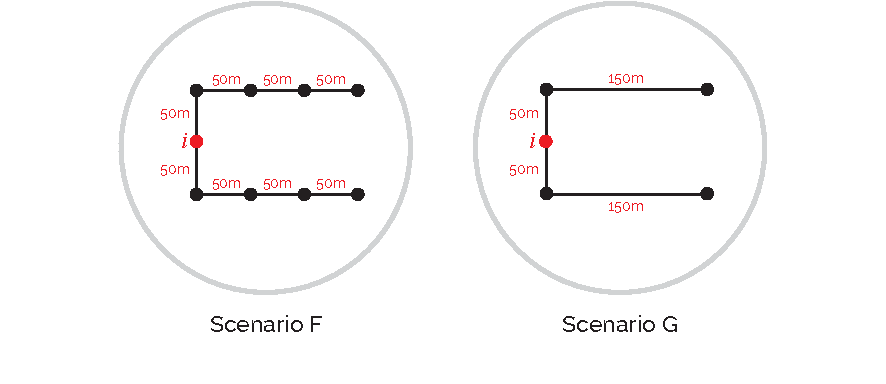
\includegraphics[width=\linewidth, keepaspectratio]{images/closeness_comparisons_length_weighted.pdf}
  \caption{Length weighted closeness formulations comparing for varied node intensities.}\label{fig:closeness_comparisons_length_weighted}
\end{figure}

\begin{table*}[htp]
  \centering
  \begin{tabular}{ r | r r }
    &
    $length\ wt.\ HC_{(i)} = \sum_{j\neq{i}}\frac{l}{d_{(i,j)}}$ &
    $Harmonic\ C_{(i)} (0, x) = \int_{0}^{x} \ln(x)\ dx$ \\
    \midrule
    \\
    Scenario F &
    $(\frac{50}{50} + \frac{50}{100} + \frac{50}{150} + \frac{25}{200})*2 = 3.92$ &
    $(simplified)\ \ln(200) * 2 = 10.60$ \\
    \\
    Scenario G &
    $(\frac{100}{50} + \frac{75}{200})*2 = 4.75$ &
    $(simplified)\  \ln(200) * 2 = 10.60$ \\
  \end{tabular}
  \caption{Length weighted closeness formulations comparing street-length weighted \emph{Harmonic Closeness} and a continuous form of \emph{Harmonic Closeness}. Continuous forms remain consistent regardless of the number of subdivisions.}\label{table:closeness_comparisons_length_weighted}
\end{table*}

Note that the continuous form of \emph{Harmonic Closeness} suggested per Equation~\ref{eq:harmonic_integral} cannot be used with \emph{geometric distance} (angular) impedances, which do not increase continuously.

As with closeness centrality, it may be preferable to use the gravity index in a continuous form. In this case, gravity is computed as the area under the curve for all reachable segments $S$ for the respective lower and upper segment bounds $a$ and $b$ at the specified impedance $\beta$:
\begin{equation}\label{eq:gravity_continuous}
  G_{(i)} = \sum_{(a, b)}^{S} \int_{a}^{b}\ f(x)\ dx = \sum_{(a, b)}^{S}\ \frac{\exp(-\beta\cdot b) -\exp(-\beta\cdot a)}{-\beta}.
\end{equation}